\question{Работа и мощность сил, приложенных к твердому телу при поступательном,
вращательном, сферическом и свободном движении твердого тела. Работа
внутренних сил твердого тела}

\subquestion{Работа и мощность сил приложенных к твердому телу при поступательном, 
вращательном и сферическом движении твёрдого тела}

\emph{Элементарная работа сил, приложенная к материальной точке, равна сумме 
элементарных работ этих сил.}
\[ 
	dA = \left( \vec{F}_1 + \vec{F}_2 + ... + \vec{F}_n \right)\cdot d\vec{r} =
	dA_1 + dA_2 + ... + dA_n)
\]

\begin{figure}[h!]
	\center
    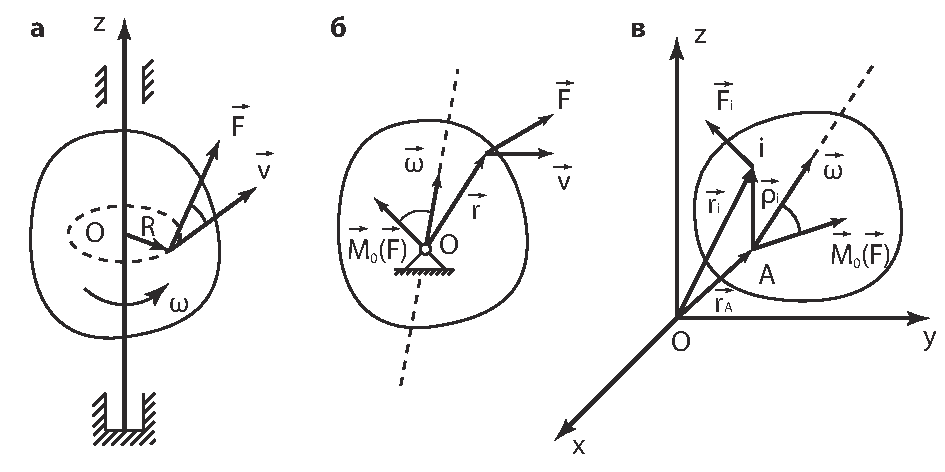
\includegraphics[width=.47\textwidth]{53_01}
    \caption{Рисунки}
    \label{pic53_01}
\end{figure}

При поступательном движении твёрдого тела его можно принять за материальную 
точку и для вычисления работы силы, приложенной к нему, применять все 
формулы для подсчёта элементарной и полной работы силы, приложенной к 
материальной точке.

При вращении твёрдого тела вокруг неподвижной оси скорость точки, где приложена 
сила \( F \) (рис.~\ref{pic53_01}а), равна \( v = \omega R \). По определению
\[ 
	dA = \vec{F}\cdot\vec{v}\,dt = Fv\cos(\widehat{\vec{F}\vec{v}})\,dt = 
	F\omega R\cos(\widehat{\vec{F}\vec{v}})\,dt.
\]
Вектор скорости лежит в плоскости, перпендикулярной оси вращения и оси \( Oz \), 
поэтому \( |F\cos(\widehat{\vec{F}\vec{v}})| = F_p \), где \( F_p \) -- модуль проекции силы
на эту плоскость. 

Следовательно, по определению момента силы относительно оси 
\( |M_z| = F_p R\), то есть \( FR\cos(\widehat{\vec{F}\vec{v}}) = \pm M_z \).

Поэтому элементарную работу силы, приложенной к телу, вращающемуся вокруг 
неподвижной оси, можно выразить так:
\[
	dA = \pm M_z\omega dt = \pm M_zd\phi
\]
где \( d\phi = \omega dt \) -- элементарный угол поворота тела.

Мощность в случае вращения твёрдого тела вокруг неподвижной оси 
вычисляется так:
\[
	N = \der{A}{t} = \pm M_z\omega.
\]

При вращении твёрдого тела вокруг неподвижной точки 
(сферическое движение) (рис.~\ref{pic53_01}б) скорость \( \vec{v} \) точки 
приложения силы \( \vec{F} \) можно выразить по 
формуле Эйлера, согласно которой \( \vec{v} = \vec{\omega}\times\vec{r} \), где 
\( \vec{r} \) -- радиус-вектор точки приложения, а \( \vec{\omega} \) -- 
мгновенная угловая скорость тела. Тогда:
\[ 
	dA = \vec{F}\cdot\vec{v}\,dt = 
	\vec{F}\cdot\left(\vec{\omega}\times\vec{r}\right)\,dt =
	\vec{\omega}\cdot\left(\vec{r}\times\vec{F}\right)\,dt
\]
так как по свойству смешанного произведения векторов 
\[
	\vec{F}\cdot\left(\vec{\omega}\times\vec{r}\right) = \vec{\omega}\cdot\left(\vec{r}\times\vec{F}\right).
\] 
Но \( \vec{r}\times\vec{F} = \vec{M}_0 \) -- момент силы относительно точки или 
центра \( O \). Поэтому 
\[ 
	dA = \vec{\omega}\cdot\vec{M}_0\,dt = 
	M_0\cdot\omega\cos(\widehat{\vec{M}_0\vec{\omega}})\,dt =
	M_\omega\omega dt = M_\omega\,d\phi,
\]
где \( d\phi \) -- элементарный угол поворота вокруг мгновенной оси 
вращения, а \( M_\omega = M_0\cos(\widehat{M_0\omega}) \) -- 
проекция вектора \( M_0 \) на направление мгновенной угловой 
скорости, которую называют \emph{моментом силы относительно мгновенной 
оси вращения}.

Мощность силы в этом случае можно выразить так:
\[ 
	N = \der{A}{t} = \vec{M}_{0}\cdot\vec{\omega} = M_\omega\cdot\omega.
\]

\subquestion{Работа и мощность сил при свободном движении. Работа внутренних сил}

В самом общем случае (рис.~\ref{pic53_01}в), когда на свободное твёрдое тело 
действует система сил \( \left( F_1, F_2, ..., F_n \right) \) скорость 
точки \( v_i \) точки тела с номером \( i \), на которую действет сила 
\( F_i \), можно выразить как 
\( \vec{v}_{i} = \vec{v}_A + \vec{\omega}\times\vec{\rho_i} \), 
где \( v_A \) -- скорость полюса \( A \), \( \rho_i \) -- радиус-вектор 
точки относительно полюса. Тогда для элементарной работы системы сил 
получим выражение:
\[ 
	dA = \sum_{i=1}^{N} \vec{F}_i
	(\vec{v}_{a} + \vec{\omega}\times\vec{\rho_i}) =
	\sum_{i=1}^{N}\vec{F}_i\cdot\vec{v}_A\,dt + 
	\sum_{i=1}^{N}\vec{F}_i\cdot(\vec{\omega}\times\vec{\rho_i})\,dt.
\]

Воспользовавшись свойствами смешанного произведения векторов, перепишем 
выражение в виде:
\[ 
	dA = \left( \sum_{i=1}^{N}\vec{F}_i \right)\cdot\vec{v}_A\,dt + 
	\left( \sum_{i=1}^{N} \vec{\rho_i}\times\vec{F}_i\right)\cdot
	\vec{\omega}\,dt = \left( \sum_{i=1}^{N}\vec{F}_i \right)\cdot\vec{v}_A\,dt
	+ \left( \sum_{i=1}^{N} \vec{M}_{i} \right)\cdot\vec{\omega}\,dt.
\]

Считая твёрдое тело неизменяемой системой материальных точек, разделим силы, 
действующие на его точки, на внешние и внутренние, то есть 
\( F_i = F^e_i + F^i_i \). Подставляя в предыдущее равенство получаем:
\[ 
	dA = \left( \sum_{i=1}^{N} \vec{F}^e_i \right)\cdot\vec{v}_A\,dt + 
	\left( \sum_{i=1}^{N} \vec{M}_{i}^e \right)\cdot\vec{\omega}\,dt +
	\left( \sum_{i=1}^{N} \vec{F}^i_i \right)\cdot\vec{v}_A\,dt + 
	\left( \sum_{i=1}^{N} \vec{M}_{i}^i \right)\cdot\vec{\omega}\,dt.
\]

В последнем выражении главный вектор и главный момент внутренних сил 
абсолютно твёрдого тела, согласно свойствам внутренних сил системы, равны нулю:
\[ 
	\sum\vec{F}^i_i = \vec{R}^i = 0,\quad 
	\sum\vec{M}_{i}^i = \vec{M}^i = 0.
\]

Следовательно, \emph{элементарная \( dA^i\) и полная работа \( A^i \), 
а также мощность \( N^i \) внутренних сил абсолютно твёрдого тела 
равна нулю.}

\newpage
